% front matter (fold)
% -----------------------------------------------
% Template for ICMC 2005
%     icmc.sty -> style file
% By Eloi Batlle (eloi@iua.upf.es), changes for 
% ICMC 2005 by Bram de Jong 
% Adapted for the ICMC 2008 by Maarten van Walstijn
% -----------------------------------------------

\documentclass{article}
\usepackage{icmc,amsmath}
\usepackage{graphicx}
\usepackage{hyperref}
\usepackage{url}
\usepackage{color}
\definecolor{black}{rgb}{0,0,0}
\hypersetup{colorlinks,urlcolor=black,linkcolor=black,citecolor=black}  
%reduces the space between the items in the itemize-environment 
\newenvironment{packed_enumerate}{
\begin{enumerate}
  \setlength{\itemsep}{1pt}
  \setlength{\parskip}{0pt}
  \setlength{\parsep}{0pt}
}{\end{enumerate}}
\newenvironment{packed_item}{
\begin{itemize}
  \setlength{\itemsep}{1pt}
  \setlength{\parskip}{0pt}
  \setlength{\parsep}{0pt}
}{\end{itemize}}

% Title.
% ------
\title{Flexible Control of Composite Parameters in Max/MSP}

% Single address
% To use with only one author or several with the same address
% ---------------
\oneauthor
    { Timothy Place,$^{a}$ Trond Lossius,$^{b}$ Alexander Refsum Jensenius,$^{c}$ Nils Peters$^{d}$ }
	{	$^{a}$ Electrotap, tim@electrotap.com\\
		$^{b}$ BEK - Bergen Center for Electronic Arts, lossius@bek.no\\
		$^{c}$ University of Oslo, a.r.jensenius@imv.uio.no\\
		$^{d}$ CIRMMT, McGill University, Montr\'eal, nils.peters@mcgill.ca } 

% front matter (end)

\begin{document}
\maketitle
\sloppy

% Hyphenations (fold)
\hyphenation{ja-mo-ma}
\hyphenation{Ramp-Unit}
\hyphenation{Ramp-Units}
\hyphenation{Function-Unit}
\hyphenation{Function-Units}
% Hyphenations (end)

%%%%%%%%%%%%%%%%%%%%%%%%%%%%%%%%%%%%%%%%%%%%%%%%%%%%%%%%%%%%%%%%%%%%%%%%%%%%%%%
%%%%%%%%%%%%%%%%%%%%%%%%%%%%%%%%%%%%%%%%%%%%%%%%%%%%%%%%%%%%%%%%%%%%%%%%%%%%%%%
%%%%%%%%%%%%%%%%%%%%%%%%%%%%%%%%%%%%%%%%%%%%%%%%%%%%%%%%%%%%%%%%%%%%%%%%%%%%%%%
\begin{abstract}
%The abstract should be placed at the top left column and should contain about 150-200 words.

% CHANGED: [TL] Added first paragraph back in. The first paragraph is to me not at all philosophical, but points to a fundamental and very real problem when working creatively with computer based media systems. This is, to me at least, the fundamental motivation why we have spent so much energy on development of how to do ramping in Jamoma.  Also, Tim says the abstract should be in the third person (so we don't use 'we' in the abstract).

Fundamental to the development of musical or artistic creative work is the ability to transform raw materials. This ability implies the facility to master many facets of the material, and to shape it with plasticity. Computer music environments typically provide points of control to manipulate material by supplying parameters with controllable values. This capability to control the values of parameters is inadequate for many artistic endeavors, and does not reflect the analogous tools and methods of artists working with physical materials.

Rather than viewing parameters in computer-based systems as single points of control, the authors posit that parameters must become more multifaceted and dynamic in order to serve the needs of artists. The authors propose an expanded notion of how to work with parameters in computer-centric environments for time-based art. A proposed partial solution to this problem is to give parameters additional properties that define their behavior. An example implementation of these ideas is presented in Jamoma. 

\end{abstract}

%%%%%%%%%%%%%%%%%%%%%%%%%%%%%%%%%%%%%%%%%%%%%%%%%%%%%%%%%%%%%%%%%%%%%%%%%%%%%%%
%%%%%%%%%%%%%%%%%%%%%%%%%%%%%%%%%%%%%%%%%%%%%%%%%%%%%%%%%%%%%%%%%%%%%%%%%%%%%%%
%%%%%%%%%%%%%%%%%%%%%%%%%%%%%%%%%%%%%%%%%%%%%%%%%%%%%%%%%%%%%%%%%%%%%%%%%%%%%%%
\section{Introduction} % (fold)
\label{sec:introduction}

% CHANGED: [TL] We want the main subject of the paper to be how to create more advanced and flexible ways of controlling parameters. The discussion of static vs. dynamic parameters is less improtant, and I also feel that it is misleading, we are only partly doing it at the moment. We are doing it at low level (jcom.parameter but we are not currenlty doing it consistently at higher levels, with exception for the mapping modules. E.g. a way of dynamically route audio signals in different directions would be required in order for us to make the claim of truly being able to create dynamic networks of modules.

% The problem of static paramater control is true for many Digital Audio Workstations (DAWs) whose overall structure is fixed. It is, however, also true of open-ended systems, such as PureData or Max/MSP. In a graphical environment, the relationships between objects and their interconnections form the algorithm that determines a tool's behavior. Within this algorithm there is typically some freedom to modify its behavior by e.g. changing coefficients. However, the objects and connections generally do not change on-the-fly as a performance is executed.

% Many of these systems, Max/MSP in particular, have provisions for breaking out of sets of static relationships through scripting. For the vast majority of users, however, mastering this task is onerous at best. By keeping these relationships fixed, the expressivity available to the user is inherently limited. 

% To address the needs for systems which are more dynamic, a possible partial solution is to treat parameters as multi-dimensional tools or objects. This paper presents the ideas of such a dynamic turn, and a prototype implemented in Jamoma,\footnote{\url{http://www.jamoma.org}} a modular framework for Max/MSP \cite{Place:2006}. 

\emph{Presets} and \emph{automation} in computer music systems can be considered possible archetypes of strategies for dynamic control of a system. Presets in their purest form are a vertical-only approach; all values are instantly set to a certain state. Automation on the other hand, in its purest form is a horizontal-only approach; a fixed stream of time-tagged values progressing over a limited amount of time to control the state of one parameter, often with interpolation from one value to the next. While presets are widely used in real-time signal processing environments, the use of automation is fundamental to linear time-based media software such as digital audio workstations and video editing software.

One obvious way of expanding the flexibility of presets is by implementing a cross-fade or gradual transition to the new preset by means of interpolation. Several works have expanded this further by presenting the set of presets as points in a dataspace and developing strategies of traversing that dataspace, creating dynamic interpolations between two or more presets \cite{Bencina:2005metasurface, Dahlstedt:2001, Momeni:2003}. This has also been extensively used by one of the authors for developing the Hipno audio plug-ins \cite{Place:2005hipno}.

Jamoma\footnote{\url{http://www.jamoma.org}} is a system for developing high-level \emph{modules} in the Max/MSP/Jitter environment \cite{Place:2006}. It implements a \emph{Model-View-Controller} (MVC) strategy, where ``objects of different classes take over the operations related to the application domain (the model), the display of the application's state (the view), and the user interaction with the model and the view (the controller).'' \cite[p.~26]{Krasner:1988}. All state management, parametric control, and automation for Jamoma is handled within the controller layer of the MVC paradigm. This forms the basis of all relationships both within a module and between different modules.

In Jamoma we are currently working towards more complex transitions of parameters in time that integrate both vertical and horizontal qualities.  This is achieved through the integration of a cuelist system. This system permits instant updates to parameters, or scripting of complex transitional progressions, introducing horizontal aspects. 

Previously, Jamoma offered possibilities of \emph{ramping} to a new value over a certain amount of time by means of linear interpolation only. Recently this has been expanded by re-implementing ramps as a combination of two new libraries.

% section introduction (end)

%%%%%%%%%%%%%%%%%%%%%%%%%%%%%%%%%%%%%%%%%%%%%%%%%%%%%%%%%%%%%%%%%%%%%%%%%%%%%%%
%%%%%%%%%%%%%%%%%%%%%%%%%%%%%%%%%%%%%%%%%%%%%%%%%%%%%%%%%%%%%%%%%%%%%%%%%%%%%%%
%%%%%%%%%%%%%%%%%%%%%%%%%%%%%%%%%%%%%%%%%%%%%%%%%%%%%%%%%%%%%%%%%%%%%%%%%%%%%%%
\section{The Composite Parameter} %(fold)
\label{sec:the_composite_parameter}

The parameter is the primary interface for a user manipulating the state of a module. In most systems, the parameter has a single task: to set a variable or coefficient. While it is straightforward to understand such a simple one-dimensional control, it does not offer the degree of nuance that, say, a sculptor has when working with clay.

In Jamoma, the parameter is expanded by adding \emph{properties} and \emph{methods} to the parameter that further refine or change its behavior \cite{Place:2008}. These behaviors themselves can be in constant fluid motion together with the value of the parameter. Some examples of parameter properties include setting a value range, filtering out repetitions, determining the type of unit used to express values, and how automation is applied.  The result is a composite parameter or \emph{node}, made up of many constituent parts rather than representing only a single value. As such it is more like a multi-dimensional tool than a single point of control.

\subsection{Properties and Methods} %(fold)
\label{sec:properties_and_methods}

We have stated that a parameter may be enhanced by the addition of \emph{properties} and \emph{methods}. A property is an aspect of the parameter which itself has a state. For example, filtering of repetitive values can be turned on or off. A method is simply a mechanism for doing something, such as refreshing the user interface for the parameter. A method, however, does not have any value to maintain.

One interesting aspect of properties, which does not apply to methods, is that properties may themselves have properties, as illustrated in Figure~\ref{fig:structure}.

\begin{figure}[ht]
\centerline{\framebox{
	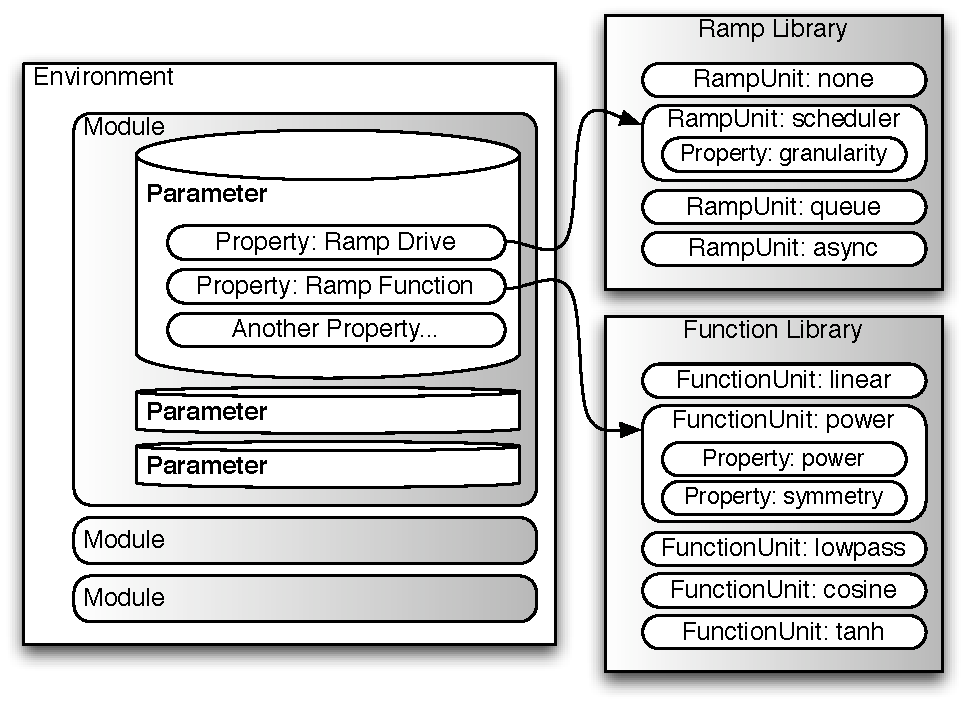
\includegraphics[width=\columnwidth]{figure-structure}}}
\caption{Parameter structure in context: Within an environment, there may be many modules. Each module may have many parameters. Each parameter may have many properties. A property may point to a dynamic entity which itself has properties, and so on.}
\label{fig:structure}
\end{figure}

% subsection properties_and_methods (end)

\subsection{Parameter Properties in Jamoma} %(fold)

Jamoma's parameter object is an implementation of the idea that properties and methods can meaningfully extend parametric control. When communicating to and from modules using the Open Sound Control protocol \cite{Wright:2003}, we use the colon separator to access the properties of the parameter as proposed in \cite{Place:2008}:

\begin{small}
\begin{verbatim}
/path/to/parameter <value>
/path/to/parameter:/property <value>
\end{verbatim}
\end{small}

Table~\ref{tab:parameter_properties} lists the currently implemented properties of the parameter object, with the path to the parameter omitted.

\begin{table}[ht]
\begin{center}
\footnotesize\noindent
\begin{tabular}{| l | p{4.5cm} |}
    \hline
    \textbf{Property or Method}          & \textbf{Description}\\ 
	\hline
	\texttt{:/value}			& Value of the parameter \\
	\hline
	\texttt{:/value/stepsize}	& Size of step taken \texttt{inc} and \texttt{dec} \\
	\hline
	\texttt{:/value/inc}		& Increase the value \\
	\hline
	\texttt{:/value/dec}		& Decrease the value \\
	\hline
	\texttt{:/value/default}	& Initial value \\
	\hline
	\texttt{:/type} 			& Type of data (int, float, etc.) \\
	\hline
	\texttt{:/priority} 		& Order for recalling values from a preset \\
	\hline
	\texttt{:/view/freeze} 		& Stops GUI updates to save CPU \\
	\hline
	\texttt{:/view/refresh} 		& Updates the GUI \\
	\hline
	\texttt{:/ramp/drive} 		& Timing mechanism for ramps \\
	\hline
	\texttt{:/ramp/function} 	& Interpolation shape for ramps \\
	\hline
	\texttt{:/repetitions} 		& Filter out repeated values \\
	\hline
	\texttt{:/range/bounds} 	& Set a low and high range \\
	\hline
	\texttt{:/range/clip} 		& What to do when the range is exceeded \\
	\hline
	\texttt{:/description} 		& Documentation \\
	\hline
	%\texttt{:/node/type} 		& ``parameter'' or ``message'' \\
	%\hline
	%\texttt{:/node/name} 		& Parameter's name \\
	%\hline
	%\texttt{:/dataspace} 		& Class of values being controlled. \\
	%\hline
	%\texttt{:/dataspace/unit/active} 	& The measurement unit used when values are sent \\
	%\hline
	%\texttt{:/dataspace/unit/native} 	& The measurement unit used by the internal algorithm \\
	%\hline
\end{tabular}
\end{center}
\caption{Selected parameter properties and methods in Jamoma}
\label{tab:parameter_properties}
\end{table}

% subsection parameter_properties_in_jamoma (end)
% section the_composite_parameter (end)

%%%%%%%%%%%%%%%%%%%%%%%%%%%%%%%%%%%%%%%%%%%%%%%%%%%%%%%%%%%%%%%%%%%%%%%%%%%%%%%
%%%%%%%%%%%%%%%%%%%%%%%%%%%%%%%%%%%%%%%%%%%%%%%%%%%%%%%%%%%%%%%%%%%%%%%%%%%%%%%
%%%%%%%%%%%%%%%%%%%%%%%%%%%%%%%%%%%%%%%%%%%%%%%%%%%%%%%%%%%%%%%%%%%%%%%%%%%%%%%
% TODO: Can we come up with a more informative title for this section?
\section{Implementation} %(fold)
\label{sec:param_implementation}

In Jamoma, the parameter is implemented as a Max external called \emph{jcom.parameter}. Within jcom.parameter, the ramping properties are implemented internally as a combination of two shared libraries called the \emph{RampLib} and \emph{FunctionLib}. The RambLib determines \emph{when} a new value is required during a ramp, while the FunctionLib determines \emph{what} the new value will be. Both of these are reconfigurable on-the-fly during performance.

%%%%%%%%%%%%%%%%%%%%%%%%%%%%%%%%%%%%%%%%%%%%%%%%%%%%%%%%%%%%%%%%%%%%%%%%%%%%%%%
\subsection{The Ramp Library} % (fold)
\label{ssec:ramplib}

Depending on the circumstance, it may be desirable to generate new interpolated values in different ways during the ramp. Several real-time signal processing environments distinguish between audio rate and control rate signals \cite{Boulanger:2000csound, McCartney:1996supercollider}. If the parameter is controlling a video processing algorithm it may be sufficient to update the value once per processed video frame \cite{Jones:2005jitter}.

The Jamoma RampLib provides a means by which to create and use \emph{RampUnits} in Jamoma.  A RampUnit is a self-contained algorithm that can slide from an existing value to a new value over a specified amount of time according to a timing mechanism. RampUnits are implemented in C++ using the TTBlue API\footnote{TTBlue is an object-oriented, reflective, application programming interface for C++, with an emphasis on real-time signal processing. \url{http://code.google.com/p/ttblue}}. Currently four such RampUnits are implemented:

\begin{itemize}
	\item \emph{none} - jumps immediately to the new value. Typically used for values where ramping is not relevant or desirable.
	\item \emph{scheduler} - uses the Max internal clock to generate new values at fixed time intervals. The timing granularity can be controlled using a property.
	\item \emph{queue} - ramps using the Max queue, updating values whenever the processor has free capacity to do so.
	\item \emph{async} - only calculates new values when requested to do so. This is typically used in video processing modules to calculate fresh values immediately before processing the next video image or matrix.
\end{itemize}

The RampLib can easily be extended with more RampUnits, and one planned extension is the implementation of audio rate ramping.

When a new ramp is started, the RampUnit internally uses a normalized ramping value increasing linearly from $0.0$ to $1.0$ over the duration of the ramp. Whenever the RampUnit is to provide a new value, it updates the normalized ramping value and passes it to a FunctionUnit as described in Section~\ref{ssec:functionlib}. The normalized value is then returned and scaled to the range defined by the start and end values for the ramp, and passed on to the module.

% subsection ramplib (end)

%%%%%%%%%%%%%%%%%%%%%%%%%%%%%%%%%%%%%%%%%%%%%%%%%%%%%%%%%%%%%%%%%%%%%%%%%%%%%%%
\subsection{The Function Library} % (fold)
\label{ssec:functionlib}

The Jamoma FunctionLib API provides normalized mappings of values $x \in [0,1]$ to $y \in [0,1]$ according to functions $y = f(x)$. Currently five functions are implemented: 

\begin{itemize}
	\item Linear: $y = x$
	\item Cosine: $y = - \frac{1}{2} \cdot cos(x \cdot \pi ) + \frac{1}{2} $
	\item Lowpass series: $y[n] = y[n-1] \cdot k + x[n] \cdot (1-k)$ \\ The feedback coefficient $k$ can be set as a property.
	\item Power function: $ y = x^{k} $. \\ The parameter $k$ can be set as a property.
	\item Hyperbolic tangent: $ y = c \cdot (\tanh(a\cdot(x-b)) - d) $ \\ The width and offset of the curve can be set as properties.  These in turn set the values of the coefficients $a$, $b$, $c$ and $d$.
\end{itemize}

The FunctionLib can easily be expanded by introducing new functions as C++ classes, also using the TTBlue API.

% TODO: We should have exponensial functions implemented by the time the final version of the paper is completed.

%The Jamoma libraries deliver a shared resource to all of the Jamoma framework for applying mathematical functions, converting units, and ramping. For example, the ramping functionality is not only implemented in parameters, but also in messages, special ramping objects, and in other places. The tools implemented in the libraries are pervasive throughout the environment.

%Each of the libraries furnish a clear programming interface so that they are easily extendable. The dynamic binding implementation in the Jamoma framework means that by simply creating one \emph{unit} (object), it is immediately available to the rest of the Jamoma environment with no additional upkeep or maintenance elsewhere in the code.

%The libraries can also be queried to find out what functionalities exist. This happens at several levels.  For example, a user may wish to find out what functions exist for doing a mathematical mapping. The FunctionLib can provide a list of available FunctionUnits. Having chosen a FunctionUnit, the user can then query to find out what additional properties (if any) the FunctionUnit has published for access. A good user interface will automate all of this querying to simply provide updated selections and options.

%Currently there are three libraries in the Jamoma framework:
%\begin{itemize}
%	\item FunctionLib: a library of FunctionUnits which map an input value to an output value
%	\item RampLib: a library of driving mechanisms (RampUnits) which use the FunctionLib to %automate value transformations over time.
%	\item DataspaceLib: a library by which a parameter or message can be given a class that describes the type of data it represents.  Values may then be set by any of a number of DataspaceUnits to allow control of a parameter in any of a number of ways.
%\end{itemize}


% section functionlib (end)

\subsection{Combinations} %(fold)
\label{sec:combinations}

\begin{figure}
\centerline{\framebox{
	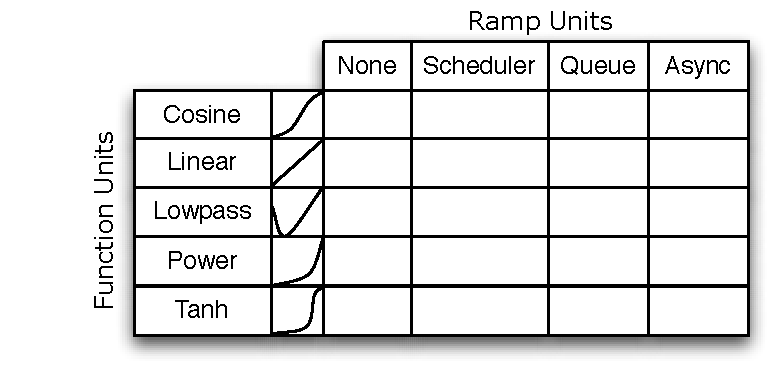
\includegraphics[width=\columnwidth]{figure-combinations}}}
\caption{The possible ramping configurations in Jamoma can be represented as the intersection of a choice on each of the x and the y axes.}
\label{fig:combinations}
\end{figure}

One of the advantages of implementing ramping as a combination of two libraries, is that any RampUnit can be combined with any FunctionUnit. Currently, with 4 RampUnits and 5 FunctionUnits implemented, this provides a total of 20 options for how to perform ramping, as illustrated in Figure~\ref{fig:combinations}.

% subsection combinations (end)
% section the_jamoma_libraries (end)


%%%%%%%%%%%%%%%%%%%%%%%%%%%%%%%%%%%%%%%%%%%%%%%%%%%%%%%%%%%%%%%%%%%%%%%%%%%%%%%
%%%%%%%%%%%%%%%%%%%%%%%%%%%%%%%%%%%%%%%%%%%%%%%%%%%%%%%%%%%%%%%%%%%%%%%%%%%%%%%
%%%%%%%%%%%%%%%%%%%%%%%%%%%%%%%%%%%%%%%%%%%%%%%%%%%%%%%%%%%%%%%%%%%%%%%%%%%%%%%
\section{Discussion and further work} % (fold)
\label{sec:discussion_and_further_work}

The proposed system for the ramping of parameter values can be understood as an extension of the well-established ADSR (attack - decay - sustain - release) envelope used in classic synthesizers to create increasingly complex developments over time. Ramps are initiated and controlled by simple OSC messages, thus combining simplicity of access with complexity and expressivity of the result.

One Jamoma module, \emph{jmod.cuelist}, loads a text-based script of \emph{event cues}, and is able to control all other modules \cite{Place:2006}. A \texttt{WAIT} syntax can set the execution of a cue on hold for a specified amount of time. Thus more complex auditive events can be created by combining parallel ramps for several parameters. Simultaneously the transitional curve for each of the parameters can be made more complex by building compound curves splicing together several ramp segments, where different functions can be used for each segment, as illustrated in Figure~\ref{fig:cuescript}.

\begin{figure}[ht]
\begin{small}
\begin{verbatim}
#######################################
CUE upAndDown
#######################################
	/path/to/parameter 0.
	/path/to/parameter:/ramp/function linear
	/path/to/parameter 1. ramp 2000
	WAIT 2000
	/path/to/parameter:/ramp/function cosine
	/path/to/parameter 0. ramp 8000
\end{verbatim}
\end{small}
\centerline{\framebox{
	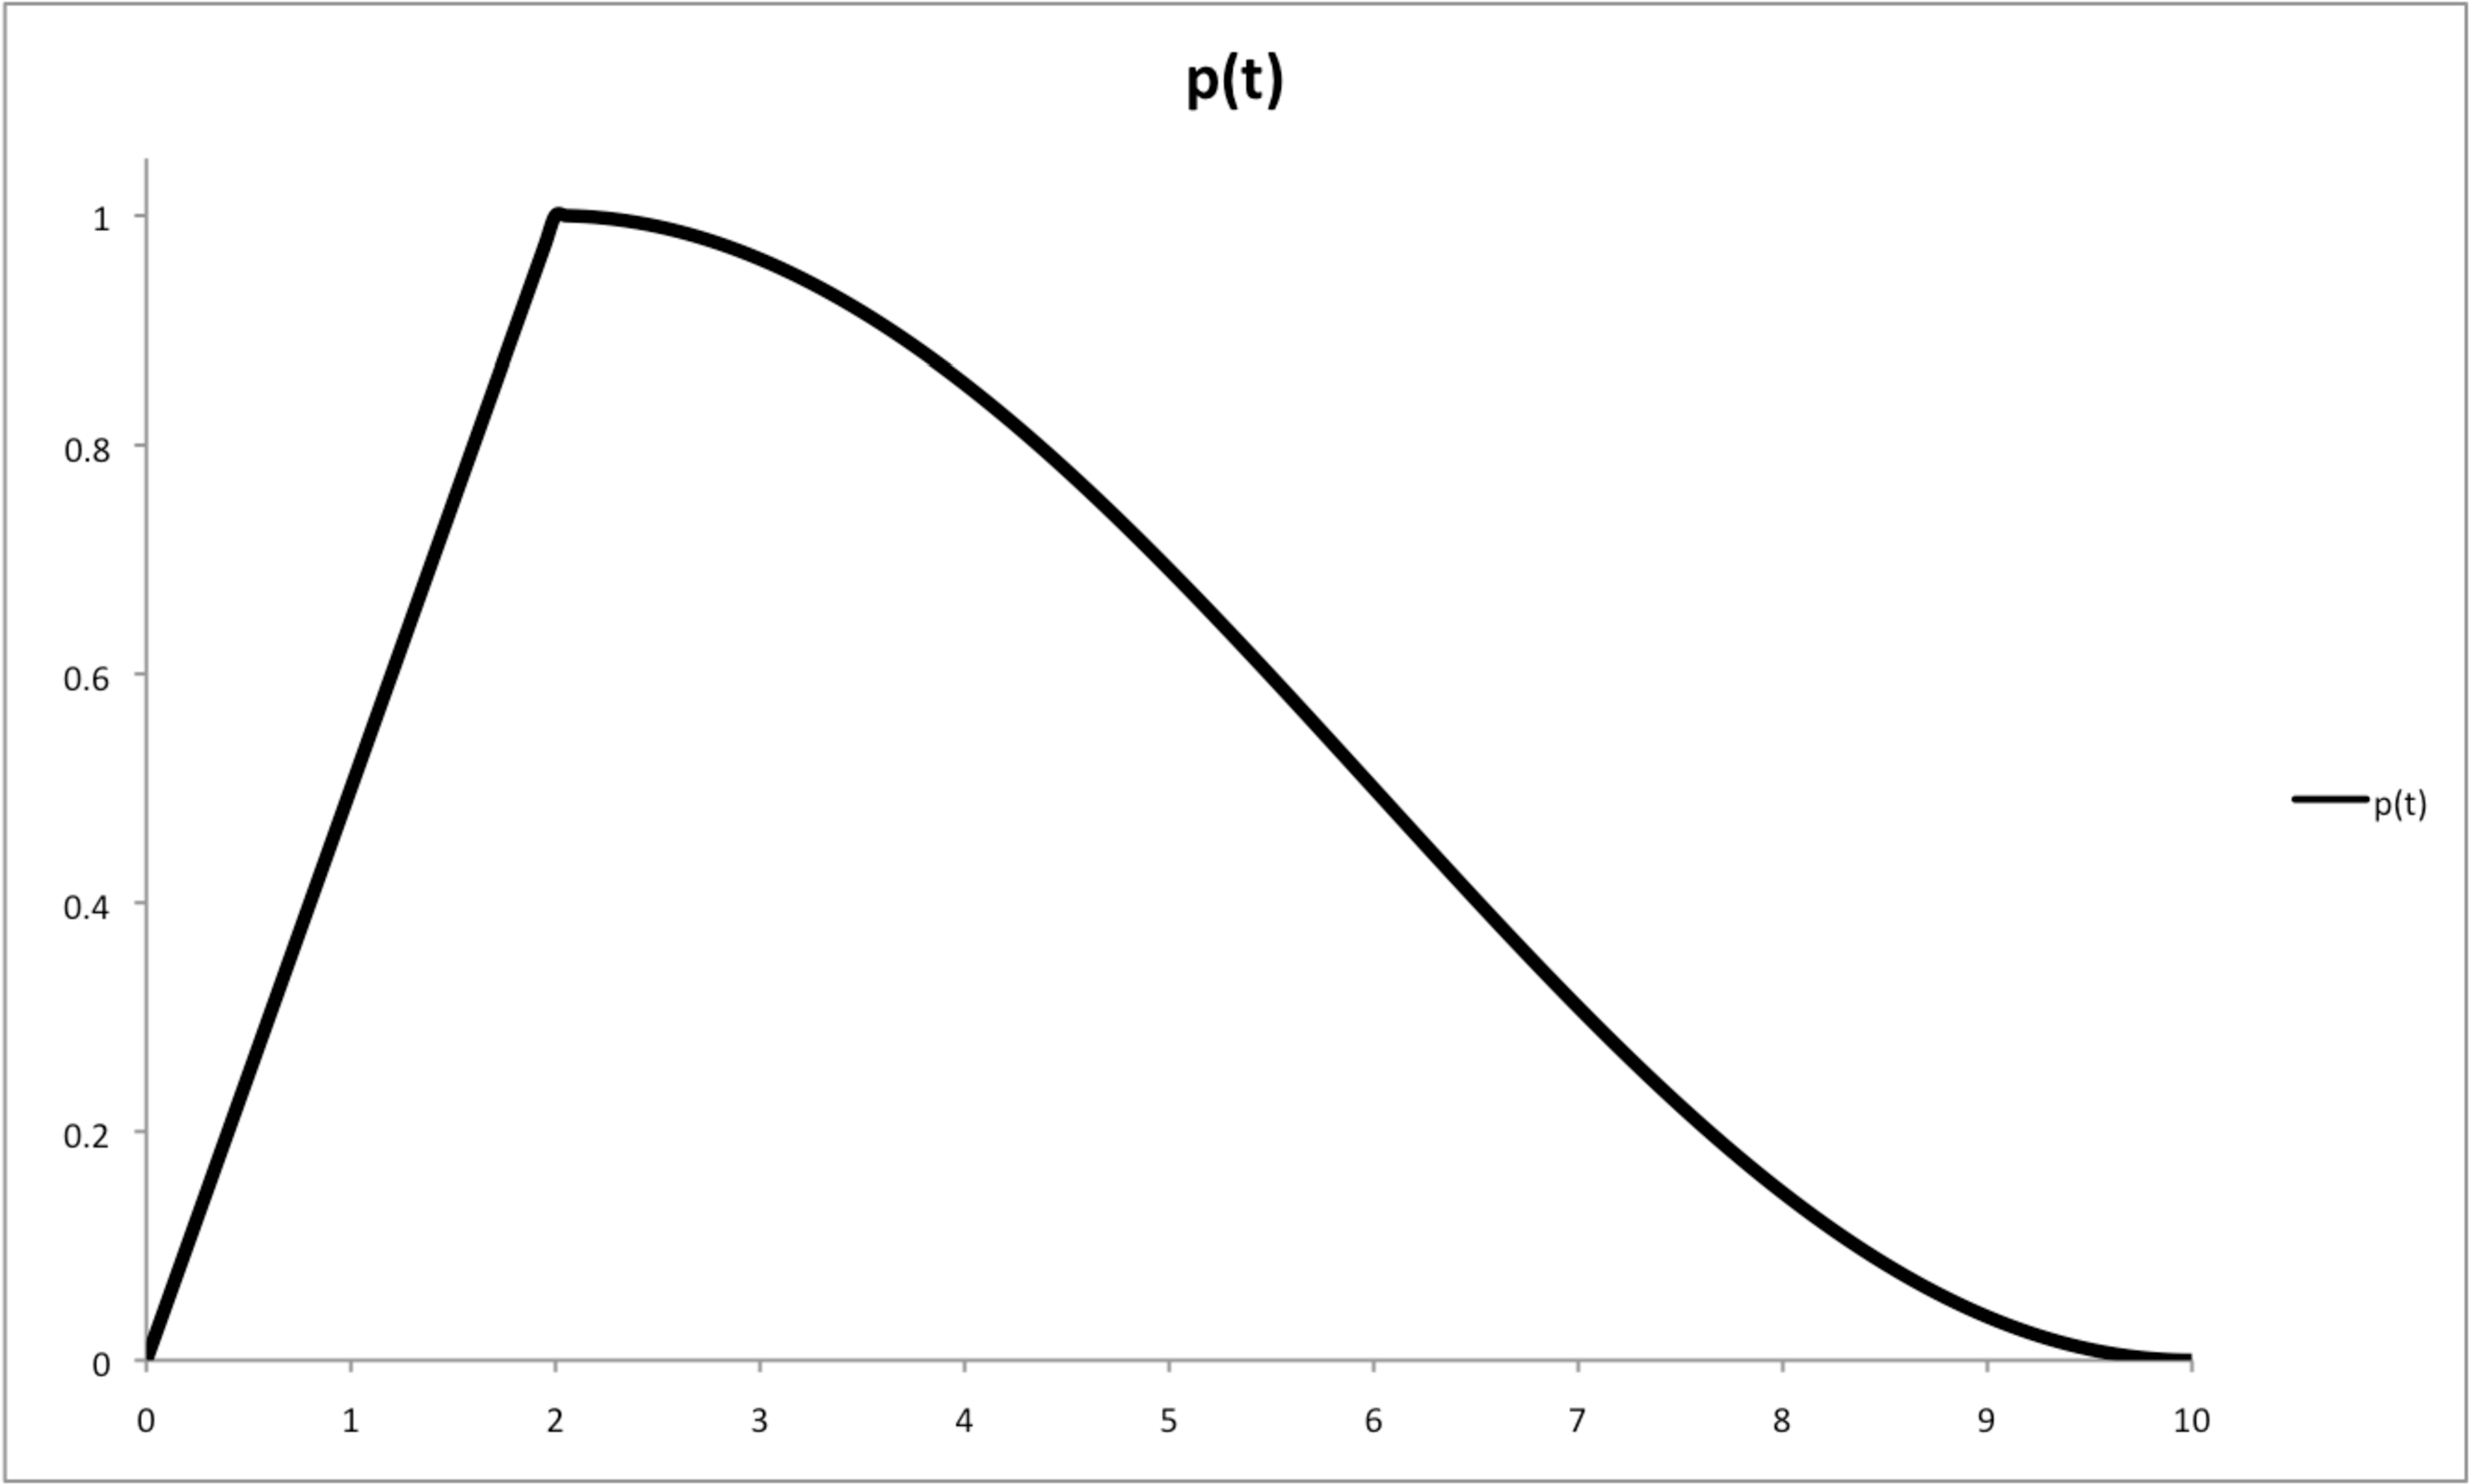
\includegraphics[width=\columnwidth]{figure-upAndDown}}}
\caption{A simple cue script. The parameter first traverses linearly from 0.0 to 1.0 in two seconds, and then returns to 0.0 in eight seconds according to a cosine function}
\label{fig:cuescript}
\end{figure}

In the discussion thus far, ramps have been implicitly understood to be \emph{goal-directed}.  That is to say that ramps are moving towards a final destination in a fixed and limited amount of time. If this assumption is relaxed, the RampLib and FunctionLib implementations can be expanded further to provide even more possibilities for continuous movement of parameter values. For instance, low frequency oscillators can be implemented as a sequence of repeating and possibly reversed ramps. If the FunctionLib is expanded by introducing stochastic functions, and ramps are permitted to be of infinite duration, the RampLib can be used to trigger new random values when required. This leads to different types of stochastic drifts and processes in time.

Presets and automation have been mentioned in Section~\ref{sec:introduction} as archetypes for strategies of dynamic control in a system. A third possible archetype for controlling a system is the use of mappings. Mappings define relationships between various components in a system that interact with each other. This creates a complex and dynamic methodology for generating not only vertical transmogrifications but gestures which develop over time \cite{Hunt:2003,Nort:2006}.

The FunctionLib can also be used outside the context of jcom.parameter. The \emph{jcom.map} Max external maps values in the input range $[a,b]$ to values in the output range $[c,d]$. The FunctionLib is used to determine the curve which shapes the mapping. This curve can be changed on-the-fly by switching between any of the available FunctionUnits. %CHAMGED: "The FunctionLib is used to determine the curve used to perform the mapping."   to "The FunctionLib is used to determine the curve which shapes the mapping." [NP]

In a similar way the RampLib can be applied outside the context of jcom.parameter for other scheduled tasks.
%CHANGED: "In a similar way the RampLib can be used outside the context of jcom.parameter for other scheduled tasks."  to "In a similar way the RampLib can be applied outside the context of jcom.parameter for other scheduled tasks."
% section discussion_and_further_work (end)


%%%%%%%%%%%%%%%%%%%%%%%%%%%%%%%%%%%%%%%%%%%%%%%%%%%%%%%%%%%%%%%%%%%%%%%%%%%%%%%
%%%%%%%%%%%%%%%%%%%%%%%%%%%%%%%%%%%%%%%%%%%%%%%%%%%%%%%%%%%%%%%%%%%%%%%%%%%%%%%
%%%%%%%%%%%%%%%%%%%%%%%%%%%%%%%%%%%%%%%%%%%%%%%%%%%%%%%%%%%%%%%%%%%%%%%%%%%%%%%
\section{Acknowledgments} % (fold)

The authors would like to thank all Jamoma developers, in particular Pascal Baltazar, for valuable contributions. A workshop hosted by iMAL Center for Digital Cultures and Technology\footnote{\url{http://imal.org/}}, Brussels, with additional support from GMEA, Centre National de Cr\'eation Musicale\footnote{\url{http://www.gmea.net}} was of particular importance in the process of developing the issues presented in this paper.

%%%%%%%%%%%%%%%%%%%%%%%%%%%%%%%%%%%%%%%%%%%%%%%%%%%%%%%%%%%%%%%%%%%%%%%%%%%%%%%
%%%%%%%%%%%%%%%%%%%%%%%%%%%%%%%%%%%%%%%%%%%%%%%%%%%%%%%%%%%%%%%%%%%%%%%%%%%%%%%
%%%%%%%%%%%%%%%%%%%%%%%%%%%%%%%%%%%%%%%%%%%%%%%%%%%%%%%%%%%%%%%%%%%%%%%%%%%%%%%
% Bibliography
\bibliographystyle{abbrv}
\bibliography{jamoma-icmc2008}  % the name of the Bibliography in this case

\end{document}
